\documentclass[a4paper, 11pt]{article}
\usepackage[margin=1.1in]{geometry}

%use the english line for english reports
%usepackage[english]{babel}
\usepackage[portuguese]{babel}
\usepackage[utf8]{inputenc}
\usepackage{indentfirst}
\usepackage{graphicx}
\usepackage{verbatim}
\usepackage{fancyhdr}
\usepackage{listings}
\usepackage{color}

\definecolor{dkgreen}{rgb}{0,0.6,0}
\definecolor{gray}{rgb}{0.5,0.5,0.5}
\definecolor{orange}{rgb}{1,0.54,0}

\lstset{frame=tb,
  language=C,
  aboveskip=3mm,
  belowskip=3mm,
  showstringspaces=false,
  columns=flexible,
  basicstyle={\small\ttfamily},
  numbers=none,
  numberstyle=\tiny\color{gray},
  keywordstyle=\color{blue},
  commentstyle=\color{dkgreen},
  stringstyle=\color{orange},
  breaklines=true,
  breakatwhitespace=true,
  tabsize=3
}

\begin{document}

\setlength{\textwidth}{16cm}
\setlength{\textheight}{22cm}

\title{\Huge\textbf{1º Trabalho Laboratorial:}\linebreak\linebreak
\Huge\textbf{Ligação de Dados}\linebreak\linebreak\linebreak
\Large\textbf{Relatório}\linebreak\linebreak
\linebreak\linebreak

\includegraphics[scale=0.1]{images/feup-logo.png}\linebreak\linebreak
\linebreak
\Large{Mestrado Integrado em Engenharia Informática e Computação} \linebreak\linebreak
\Large{Redes de Computadores}\linebreak
}

\author{\textbf{Turma 1 Grupo 2:}\\
\linebreak\\
André Cruz - 201503776 \\
Bruno Piedade - 201505668 \\
Edgar Carneiro - 201503748 \\
\linebreak\linebreak \\
 \\ Faculdade de Engenharia da Universidade do Porto \\ Rua Roberto Frias, s\/n, 4200-465 Porto, Portugal \linebreak\linebreak
\linebreak\linebreak\vspace{1cm}}

\maketitle
\thispagestyle{empty}

%************************************************************************************************
%************************************************************************************************

\newpage

%Todas as figuras devem ser referidas no texto. %\ref{fig:codigoFigura}
%
%%Exemplo de código para inserção de figuras
%%\begin{figure}[h!]
%%\begin{center}
%%escolher entre uma das seguintes três linhas:
%%\includegraphics[height=20cm,width=15cm]{path relativo da imagem}
%%\includegraphics[scale=0.5]{path relativo da imagem}
%%\includegraphics{path relativo da imagem}
%%\caption{legenda da figura}
%%\label{fig:codigoFigura}
%%\end{center}
%%\end{figure}
%
%
%\textit{Para escrever em itálico}
%\textbf{Para escrever em negrito}
%Para escrever em letra normal
%``Para escrever texto entre aspas''
%
%Para fazer parágrafo, deixar uma linha em branco.
%
%Como fazer bullet points:
%\begin{itemize}
	%\item Item1
	%\item Item2
%\end{itemize}
%
%Como enumerar itens:
%\begin{enumerate}
	%\item Item 1
	%\item Item 2
%\end{enumerate}
%
%\begin{quote}``Isto é uma citação''\end{quote}

\tableofcontents

\newpage

%Sumário
\section{Sumário}
\normalsize 

Este trabalho foi realizado no âmbito da cadeira de Redes de Computadores, e era pedido aos alunos a implementação de um protocolo de comunicação assíncrona para a transmissão de um ficheiro através de uma Porta Série RS-232.

As principais conclusões obtidas no desenvolvimento do projeto foram que o protocolo implementado foi compreensivo o suficiente para o objetivo de transmitir ficheiros com recuperação de erros e escala conforme a teoria lecionada nas aulas teóricas. O protocolo executa com cerca de 77\% de eficácia, como podemos ver pelas estatísticas geradas.

%1. Introdução
\section{Introdução}

O trabalho tinha como objetivo a implementação de um protocolo de ligação de dados, de acordo como uma especificação fornecida, através de um guião. Era também pedido aos alunos que desenvolvessem uma simples aplicação, de forma a testar o protocolo implementado.

O Relatório encontra-se dividido em diversas secções, nas quais se pode encontrar a seguinte informação:
\begin{itemize}
	\item \textbf{Arquitetura}, onde são descriminados os diferentes blocos funcionais e interfaces.
	\item \textbf{Estrutura do código}, apresentando as API's, principais estruturas de dados, principais funções e a sua relação com a arquitetura.
	\item \textbf{Casos de uso principais}, onde são identificados os principais casos de uso e as suas sequências de chamada de funções.
	\item \textbf{Protocolo de ligação lógica}, identificando os principais aspetos funcionais, bem como a descrição da estratégia de implementação.
	\item \textbf{Protocolo de aplicação},  identificando os principais aspetos funcionais, bem como a descrição da estratégia de implementação.
	\item \textbf{Validação}, descrevendo os testes efetuados.
	\item \textbf{Eficiência do protocolo de ligação de dados}, onde é realizada a caracterização estatística da eficiência do protocolo implementado.
	\item \textbf{Conclusões}, onde é feita uma tese da informação apresentada nas secções anteriores, bem como uma reflexão sobre os objetivos de aprendizagem alcançados.
\end{itemize}

%2.Arquitetura
\section{Arquitetura}

\large\textbf{Blocos Funcionais}\\
\normalsize 

No Trabalho é possível distinguir a existência de duas camadas bem definidas:  a camada do protocolo de ligação de dados - \textit{LinkLayer} - e a camada da aplicação - \textit{AplicationLayer}.
Os ficheiros \textit{LinkLayer.h} e  \textit{LinkLayer.c} representam a camada de ligação de dados. Os ficheiros \textit{AplicationLayer.h, AplicationLayer.c, Packets.h} e \\texit{ Packets.c} representam a camada da aplicação.

A camada de ligação de dados é a camada responsável pelo estabelecimento de ligação e, portanto, tem todas as funções que asseguram a consistência do protocolo, como o tratamento de erros, envio de mensagens de comunicação, entre outros. É também nesta camada que a interação com a porta série é feita, nomeadamente, a sua abertura, a escrita e leitura desta e o seu fecho.

A camada da aplicação é responsável pela envio e receção de ficheiros, segmentando o ficheiro a enviar em tramas de tamanho definível pelo utilizador. Esta camada faz uso da interface da camada de ligação de dados, chamando as suas funções para o envio e receção de segmentos do ficheiro a receber / enviar. A camada da aplicação é subdividida em duas subcamadas, dai o uso dos ficheiros \textit{AplicationLayer.h} e \textit{AplicationLayer.c} para representar a camada mais abstrata, responsável pelo envio do ficheiro e a receção do ficheiro, e que faz uso da camada menos abstrata, representada nos ficheiros  \textit{Packets.h} e \textit{Packets.c}, que é responsável pela segmentação do ficheiro em pacotes e envio de pacotes de controlo e informação.\\

\large\textbf{Interface}\\
\normalsize

Na interface da linha de comandos é permitido ao utilizador correr o programa usando o mesmo binário, independentemente de ser o recetor ou o emissor.
É necessário o utilizador especificar se será o emissor / recetor, qual o Serial Port a ser usado e, no caso do recetor, qual o ficheiro a transmitir. No entanto, existem parâmetros opcionais que permitem definir outras definições relacionadas com a transmissão de informação, tais como: \textit{baudrate}, tamanho dos segmentos de informação, número de tentativas no reenvio de tramas e tempo esperado até ao reenvio de uma trama.
Assim, a aplicação pode correr com valores inseridos pelo utilizador, ou com os seus valores por defeito.

%3.Estrutura do código
\section{Estrutura do Código}

\large\textbf{\textit{Application Layer}}\\
\normalsize

Os ficheiros \textit{AplicationLayer.h} e \textit{AplicationLayer.c}, representantes da subcamada mais abstrata da camada da aplicação, fazem uso de uma estrutura de dados que guarda o descritor do ficheiro da porta série, o nome do ficheiro a ser transmitido, o tamanho máximo de mensagem a ser transmitido e ainda o tipo de conexão a ser usado - emissor ou recetor.

\begin{lstlisting}[language=C]
typedef struct {
    int fd; // serial port's file descriptor
    char * fileName;
    ConnectionType type;
    int maxDataMsgSize;
} ApplicationLayer;
\end{lstlisting}

As principais funções desta subcamada são:

\begin{lstlisting}[language=C]
int initApplicationLayer(const char * port, int baudrate, int timeout, int numRetries, ConnectionType type, int maxDataMsgSize, char * file);
void destroyApplicationLayer();
int sendFile();
int receiveFile();
\end{lstlisting}

Os ficheiros \textit{Packets.h} e \textit{Packets.c}, representantes da subcamada menos abstrata da camada da aplicação, fazem uso de três estruturas de dados: a estrutura \textit{Packet} que guarda um apontador para a informação, e o tamanho dessa informação; a estrutura \textit{DataPacket]} que guarda o número sequencial do pacote a ser enviado, o seu tamanho e o apontador para essa informação; a estrutura \textit{ControlPacket} que guarda o tipo de pacote de Controlo - inicio ou fim -, o nome do ficheiro, o tamanho do ficheiro e o número de argumentos do pacote de controlo.

\noindent\begin{minipage}{.22\textwidth}
\begin{lstlisting}[frame=tlrb]
typedef struct {
    uchar * data;
    uint size;
} Packet;
\end{lstlisting}
\end{minipage}\hfill
\begin{minipage}{.22\textwidth}
\begin{lstlisting}[frame=tlrb]
typedef struct {
    uchar seqNr;
    uint size;
    uchar * data;
} DataPacket;
\end{lstlisting}
\end{minipage}\hfill
\begin{minipage}{.4\textwidth}
\begin{lstlisting}[frame=tlrb]
typedef struct {
    PacketType type;
    char fileName[MAX_FILE_NAME];
    uint fileSize;
    uint argNr;
} ControlPacket;
\end{lstlisting}
\end{minipage}

As principais funções desta subcamada são:

\begin{lstlisting}[language=C]
int sendDataPacket(int fd, DataPacket * src);
int sendControlPacket(int fd, ControlPacket * src);
int receiveDataPacket(int fd, DataPacket * dest);
int receiveControlPacket(int fd, ControlPacket * dest);
\end{lstlisting}

\large\textbf{\textit{Link Layer}}\\
\normalsize

A camada da ligação de dados é representada através de uma estrutura de dados onde é guardado a porta série utilizada, o \textit{baudrate} utilizado, o número de sequência da trama esperada, tempo esperado até ao reenvio de uma trama, e o número de tentativas de reenvio de uma trama.

\begin{lstlisting}[language=C]
typedef struct {
	char port[MAX_PORT_NAME];
	int baudRate;
	uint seqNumber;
	uint timeout;
	uint numRetries;
} LinkLayer;
\end{lstlisting}

As principais funções desta camada são:

\begin{lstlisting}[language=C]
int initLinkLayer(int porta, int baudRate, uint timeout, uint numTransmissions);
int openSerialPort();
int llopen(ConnectionType type);
int llclose(int fd);
int llwrite(int fd, uchar ** buffer, int length);
int llread(int fd, uchar ** buffer);
\end{lstlisting}

%4. Casos de uso principais
\section{Casos de uso principais}

Existem dois casos de uso principais bem distintos: correr o programa como emissor ou correr o programa como recetor. Em cada um destes casos é possível correr o programa usando o mesmo binário, apenas dependendo os argumentos usados na chamada do programa, sendo estes:

\begin{lstlisting}[language=C]
	printf("Usage:\t%s <SerialPort> <r/w> <FILE_NAME> [BAUDRATE] [DATA_BYTES] [NUM_RETRIES] [TIMEOUT]\n", progName);
	printf("Arguments between [ ] are optional\n");
\end{lstlisting}

No caso em que o programa é executado como \textbf{recetor} a sequência de chamada de funções, considerando as de maior relevância, é:
\begin{itemize}
	\item \textbf{receiveFile}, que tem como objetivo receber o ficheiro indicado e que faz uso de funções como a \textbf{receiveControlPacket}, \textbf{receiveDataPacket}, \textbf{llopen} e \textbf{llclose}.
	\item \textbf{receiveControlPacket}, que tem como objetivo enviar um pacote de controlo, do tipo \textit{START} no início da transmissão e do tipo \textit{END} no fim da transmissão, e que faz uso de funções como \textbf{fillControlPacketArg} e \textbf{llread}.
	\item \textbf{receiveDataPacket},  que tem como objetivo enviar um pacote de informação, e que faz uso de funções como \textbf{llread}.
	\item \textbf{fillControlPacketArg}, que tem como objetivo preencher os argumentos de um control packet, com informação recebida.
	\item \textbf{llread}, que tem como objetivo ler da Porta Série informação, aplicando-lhe \textit{Byte Destuffing} e \textit{Deframing}. Faz uso das funções \textbf{byteDestuffing, deframingInformation, sendControlFrame} e \textbf{read}.
\end{itemize}

No caso em que o programa é executado como \textbf{emissor} a sequência de chamada de funções, considerando as de maior relevância, é:
\begin{itemize}
	\item \textbf{sendFile}, que tem como objetivo enviar o ficheiro indicado e que faz uso de funções como a \textbf{sendControlPacket}, \textbf{sendDataPacket}, \textbf{llopen} e \textbf{llclose}.
	\item \textbf{sendControlPacket}, que tem como objetivo enviar um pacote de controlo, do tipo \textit{START} no início da transmissão e do tipo \textit{END} no fim da transmissão, e que faz uso de funções como \textbf{makeControlPacket} e \textbf{llwrite}.
	\item \textbf{sendDataPacket},  que tem como objetivo enviar um pacote de informação, e que faz uso de funções como \textbf{makeDataPacket} e \textbf{llwrite}.
	\item \textbf{makeControlPacket}, que tem como objetivo criar um pacote de controlo.
	\item \textbf{makeDataPacket}, que tem como objetivo criar um pacote de informação.
	\item \textbf{llwrite}, que tem como objetivo escrever para a Porta Série a informação recebida como argumento, após aplicar uma \textit{frame} e \textit{Byte Stuffing} à informação. Faz uso das funções \textbf{framingInformation, byteStuffing, readControlFrame} e \textbf{write}.
\end{itemize}

As funções de mais baixo nível, associadas à camada da ligação de dados, são usadas quer pelo emissor quer pelo recetor, sendo estas:
\begin{itemize}
	\item \textbf{llopen}, que tem como objetivo abrir a ligação da Porta Série. Faz uso das funções \textbf{openSerialPort, sendControlFrame} e \textbf{readControlFrame}.
	\item \textbf{llclose}, que tem como objetivo terminar a ligação da Porta Série. Faz uso das funções \textbf{llcloseTransmitter, llcloseReceiver} - conforme seja Emissor ou Recetor - e \textbf{close}.
	\item \textbf{sendControlFrame}, que tem como objetivo enviar uma trama de controlo. Faz uso das funções \textbf{createControlFrame} e \textbf{write}.
	\item \textbf{readControlFrame}, que tem como objetivo receber uma trama de controlo. Faz uso da função \textbf{readFromSerialPort}.
\end{itemize}

%5. Protocolo de ligação lógica
\section{Protocolo de ligação lógica}

 A camada de ligação de dados é a camada de mais baixo nível e é a camada responsável pela interação direta com a Porta Série. Algumas das funcionalidades implementada por esta camada são: abertura e fecho da Porta Série; escrita de um tramas de informação e controlo; leitura de um tramas de informação e controlo; criação de tramas de controle; \textit{byte stuffing} e \textit{byte destuffing} de uma trama; \textit{framing } e \textit{deframing} de uma trama.

A nível da API da camada de ligação de dados foram implementadas as quatro funções previstas: \textbf{llopen, llclose, llread} e \textbf{llwrite}.\\

A função \textbf{llopen} é responsável por estabelecer a ligação através da Porta Série. Faz recurso à função \textbf{openSerialPort} que abre a Porta Série e configura uma nova \textit{struct termios}. De seguida, e segundo o protocolo especificado no guião, envia uma trama de controlo do tipo SET e espera pela receção de uma trama de controlo do tipo UA, no caso do emissor, e faz o processo oposto no caso do recetor - espera pela receção de uma trama de controlo do tipo SET e após a sua receção envia uma trama de controlo do tipo UA.

A função \textbf{llclose} é responsável pelo término da ligação estabelecida através da Porta Série. Segundo o protocolo especificado no guião, o término da ligação é realizado através do envio de uma trama de controlo do tipo DISC por parte do emissor,  recessão do DISC por parte do recetor, envio de uma trama também do tipo DISC por parte do recetor, receção do DISC enviado pelo recetor, envio de uma trama de controlo do tipo UA por parte do emissor, receção do UA por parte do recetor. Após a verificação deste protocolo de terminação, é reposta a \textit{struct termios} anterior à configurada pela função \textit{llopen} e fecha-se a ligação usando o descritor de ficheiro da Porta Série.

A função \textbf{llread} é responsável pela leitura de informação da Porta Série, sendo que irá aplicar \textit{destufffing} e \textit{deframing} à trama recebida. Se ocorrer um erro no \textit{destuffing} ou um erro na \textit{frame} que não seja no \textit{BCC2} a trama é descartada, ficando assim à espera de uma nova trama. Se houver um error, e for no \textit{BCC2}, a trama é descartada, o recetor continua a espera de uma nova trama, mas envia um rama de controle do tipo REJ. Se a trama for corretamente recebida, esta é retornada e o recetor envia uma trama de controle do tipo RR.

A função \textbf{llwrite} é responsável pelo envio de informação através da Porta Série. Esta recebe a mensagem a enviar da camada superior e aplica-lhe \textit{framing} e \textit{stuffing}.
De seguida, tenta escrever a trama, sendo que se não receber uma resposta do tipo RR durante um intervalo de tempo previamente definido - \textit{default} é 3 segundos - este reenvia a trama. O reenvio da trama é feito um número de vezes previamente definido - \textit{default} é 3 tentativas. Se ao fim desse número de tentativas não tiver obtido sucesso, retorna erro.\\

\textbf{Consultar \underline{Anexo II} para extratos de código.}

%6. Protocolo de aplicação
\section{Protocolo de aplicação}

A camada de aplicação é a camada de alto nível responsável pelo processo de envio e receção do ficheiro fonte fazendo uso do API disponibilizado pela camada ligação de dados. As funcionalidades implementadas por esta camada são: inicializar a ligação; ler o ficheiro fonte e dividi-lo em pacotes de dados (caso seja emissor); reconstruir o ficheiro fonte a partir de pacotes de dados (caso seja recetor); receber e enviar os pacotes; terminar a ligação.\\

Para gerir a interação com os pacotes de dados foi desenvolvido o API (Packet.c).

Em relação aos pacotes de dados: 
A função \textbf{makeDataPacket} que cria o pacote de dados a partir da informação original do ficheiro fonte; \textbf{sendDataPacket} que envia o pacote de dados utilizando llwrite; \textbf{receiveDataPacket} que recebe o pacote de dados utilizando llread e recolhe a informação do ficheiro fonte.

Em relação aos pacotes de controlo:
A função \textbf{makeControlPacket} que cria o pacote de controlo; \textbf{sendControlPacket} que envia o pacote de controlo utilizando \textit{llwrite}; \textbf{receiveControlPacket} que recebe o pacote utilizando \textit{llread}.\\

Foram implementadas as seguintes funções:
\begin{itemize}
	\item A função \textbf{sendFile} (utilizado no caso do emissor) é responsável por inicializar a ligação, ler o ficheiro fonte e dividi-lo em pacotes de dados, enviar os mesmos e terminar a ligação. Faz recurso a 3 funções do API da camada de ligação de dados: \textit{llopen, llwrite} e \textit{llclose} e API de pacotes.
	\item A função \textbf{receiveFile} (utilizado no caso do recetor) é responsável por inicializar a ligação, ler os pacotes de dados, reconstruir o ficheiro fonte utilizando os mesmos e terminar a ligação. Faz recurso a 3 funções do API da camada de ligação de dados: \textit{llopen, llread} e \textit{llclose} e API de pacotes.
\end{itemize}

\textbf{Consultar \underline{Anexo III} para extratos de código.}

%7. Validação
\section{Validação}

Para validação do programa desenvolvido, e para garantir que funcionava de acordo com o protocolo especificado, foram realizados constantemente testes durante o desenvolvimento do programa e também na sua demonstração. Foram testados ficheiros de diferentes tamanhos e enviados com diferentes baudrates e diferentes tamanhos de pacotes de informação. Foram realizados, simultaneamente com os testes já referidos, testes de interrupção da comunicação na Porta Série e testes de introdução de erros através do curto-circuito existente nas portas séries. Todos testes terão sido também realizados na presença do professor, aquando do momento de avaliação.

%8. Eficiência do protocolo de ligação de dados
\section{Eficiência do protocolo de ligação de dados}

\textbf{Variável: Tamanho da trama I}\\
Usando um \textit{baudrate} constante de 115200 e uma imagem de tamanho constante 80942 \textit{bytes}, fazendo variar o tamanho da trama I, obteve-se:
\begin{figure}[h!]
\begin{center}
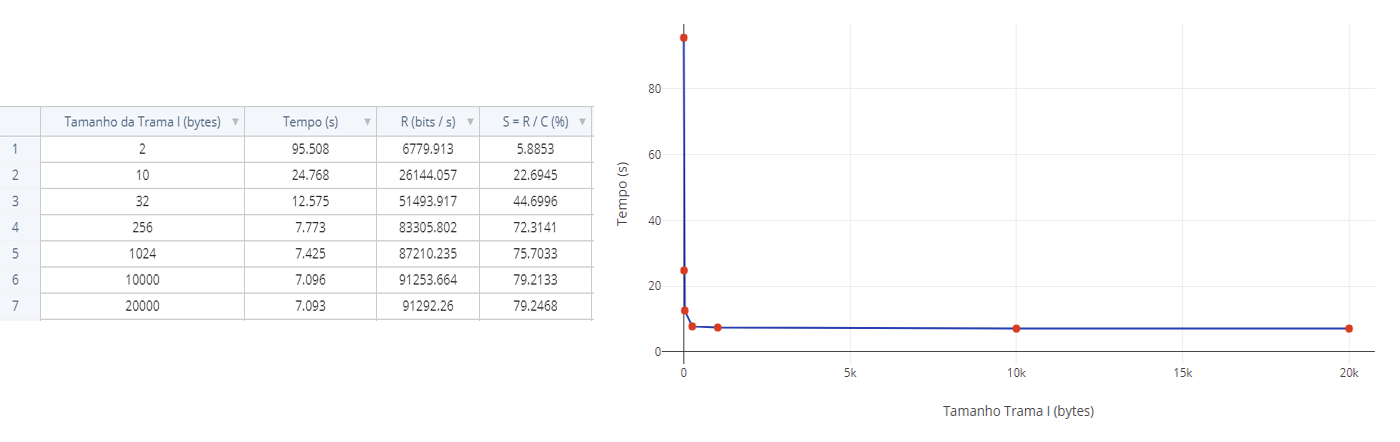
\includegraphics[scale=0.4]{images/TamanhoTrama.png}
\end{center}
\end{figure}

Após a análise dos resultados obtidos e do gráfico podemos verificar uma relação inversamente proporcional entre o Tamanho da Trama I e o Tempo Total de transferência do ficheiro. Para valores muito pequenos de trama, verifica-se grandes diferenças temporais - aumento de 8 bytes na trama de 2 bytes para 10 bytes, reduz o tempo total em cerca de 70s. Para valores grandes de trama, grandes diferenças têm pouca implicação no tempo de transferência - tramas de 10000 bytes demoram apenas mais  3ms a transferir que tramas de 20000 bytes. Verifica-se também pela análise da eficiência (S), que à medida que o tamanho da trama I aumenta, este aproxima-se do valor teórico, sendo o valor máximo obtido 79.25\%.\\

\textbf{Variável: Capacidade da ligação}\\
Usando uma imagem de tamanho constante 80942 \textit{bytes} e um tamanho de trama I constante de valor 256, fazendo variar o \textit{baudrate}, obteve-se:
\begin{figure}[h!]
\begin{center}
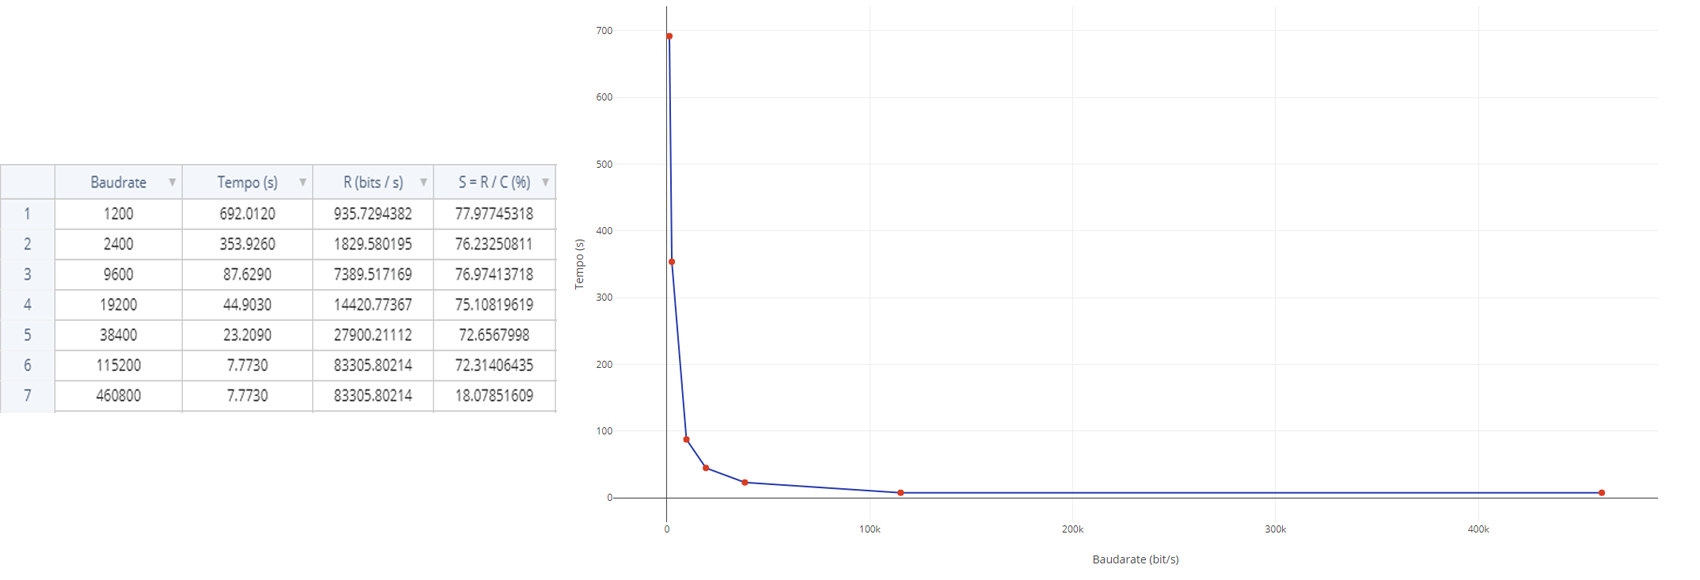
\includegraphics[scale=0.35]{images/Baudrate.png}
\end{center}
\end{figure}

Após a análise dos resultados obtidos e do gráfico podemos verificar uma relação inversamente proporcional entre o  I e o Tempo Total de transferência do ficheiro. Quanto menor o baudrate, maior o tempo de transferência.  Para valores muito pequenos de baudrate, verifica-se grandes diferenças no tempo - aumento do baudrate de 1200 para 2400, reduz o tempo total em cerca de 340 segundos. Para valores muito grandes de trama, grandes diferenças têm pouca implicação no tempo de transferência - baudrate de  115200 demora o mesmo tempo (medido até aos milisegundos) que o baudrate de 460800. Pode-se também verificar, pela análise da eficiência (S), que à medida que o tamanho da trama I aumenta, este aproxima-se do valor téorico, sendo o valor máximo obtido 77.97\%\\.

\textbf{Variável: Tempo de Propagação}\\
Usando uma imagem de tamanho constante 80942 \textit{bytes}, um tamanho de trama I constante de valor 256 e um \textit{baudrate} constante de 460800, fazendo variar o tempo de processamento de cada trama recebida, obteve-se:
\begin{figure}[h!]
\begin{center}
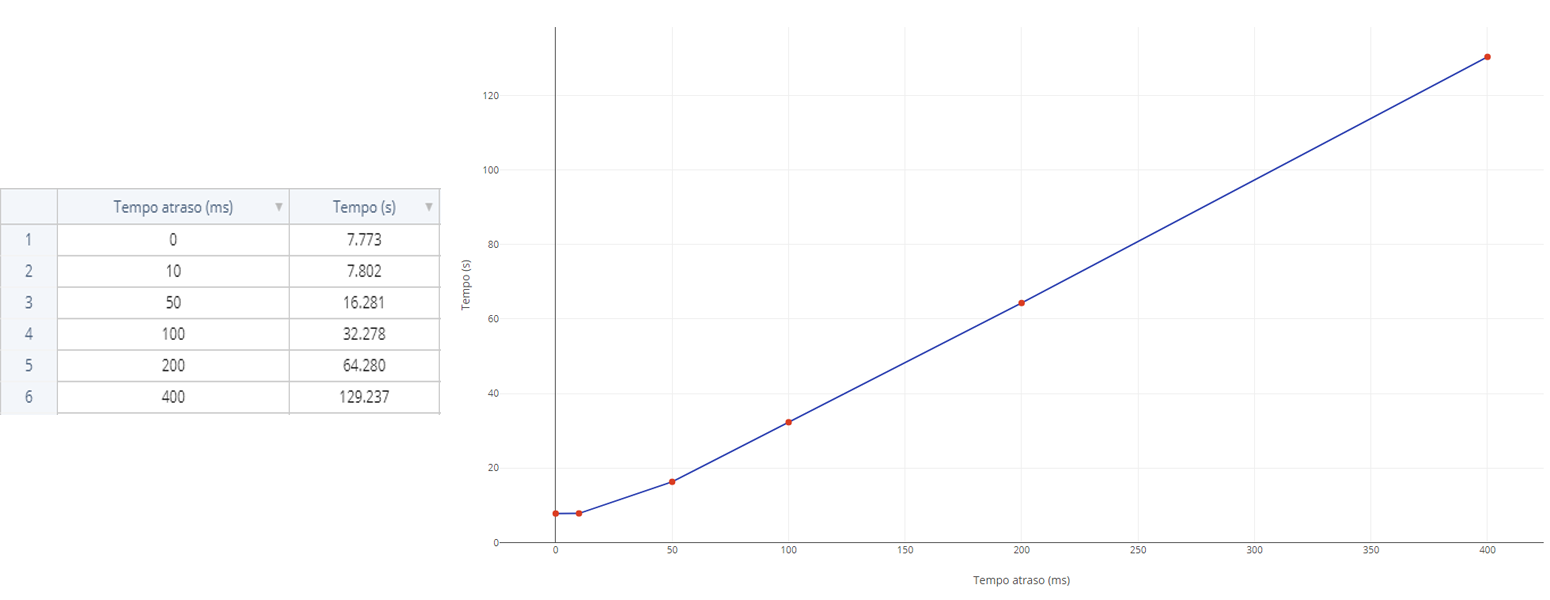
\includegraphics[scale=0.3]{images/TProp.png}
\end{center}
\end{figure}

Após a análise dos resultados obtidos e do gráfico podemos verificar uma relação diretamente proporcional entre o Tempo de Propagação e o Tempo Total de transferência do ficheiro. Assim, como era teoricamente esperado, o tempo de propagação afeta linearmente o tempo de transferência do ficheiro.

\textbf{Variável: \textit{Frame Error Ratio}}\\
Usando uma imagem de tamanho constante 80942 \textit{bytes}, um tamanho de trama I constante de valor 256 e um \textit{baudrate} constante de 460800, fazendo variar a probabilidade de ocorrência de erros no cabeçalho das tramas I, obteve-se:
\begin{figure}[h!]
\begin{center}
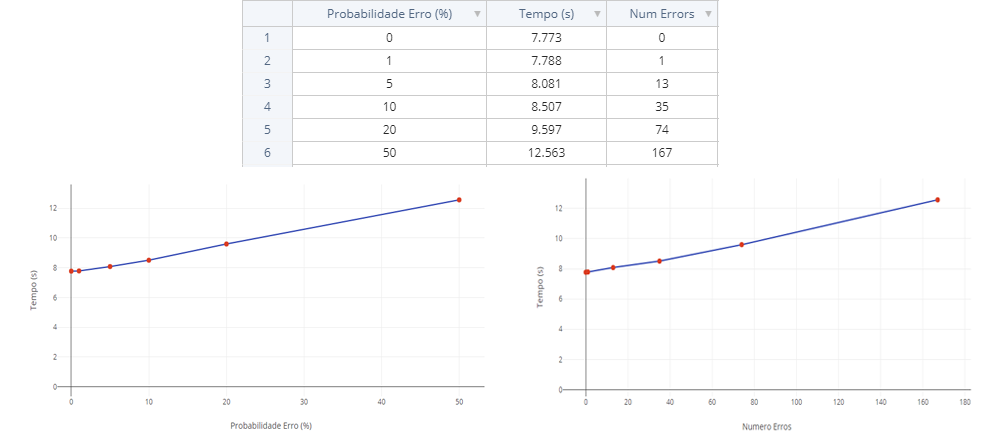
\includegraphics[width=13cm, height= 4.6cm]{images/FER.png}
\end{center}
\end{figure}

Após a análise dos resultados obtidos e do gráfico podemos verificar a semelhança com uma relação diretamente proporcional entre a probabilidade de erros no cabeçalho da trama e o Tempo Total de transferência do ficheiro. De destacar que a introdução de erros na \textit{frame} é feita através de interferência no cálculo do \textit{BCC2} dai raramente se verificar um aumento excessivo no tempo de transferência, pois o recetor deteta erros no \textit{BCC2} e responde com uma trama de controlo do tipo \textit{REJ}, não fazendo a aplicação recorrer ao \textit{timeout}.


%9. Conclusões
\section{Conclusões}

O protocolo implementado pode ser divido em duas camadas: \textit{LinkLayer} e \textit{ApplicationLayer}. A \textit{LinkLayer} como sendo a camada de mais baixo nível e fazendo iteração direta com a porta série e a \textit{ApplicationLayer} como sendo a camada de mais alto nível e que faz uso da API da \textit{LinkLayer} para enviar / receber o ficheiro. O protocolo foi implementado com robustez a erros e interrupções, conseguindo em ambos casos retomar a transferência com sucesso. A eficiência do protocolo é de cerco de 77\%, aproximando-se bastante dos valores teóricos esperados.

No final, o grupo conclui que a implementação de protocolos representa um desafio, principalmente devido aos mecanismos de deteção de erros e de recuperação. Ainda assim, o grupo considera ter dominado os conceitos teóricos implícitos no trabalho, tais como o uso de \textit{stuffing, destuffing, framing, deframing} e \textit{Stop\&Wait} com \textit{sequence numbers}. O grupo considera que o desenvolvimento do protocolo consolidou os conhecimentos teóricos previamente adquiridos.

\newpage

%Anexo I
\section{Anexo I}

\huge\textbf{main.c}
\begin{lstlisting}[language=C]
#include <sys/types.h>
#include <sys/stat.h>
#include <fcntl.h>
#include <termios.h>
#include <stdio.h>
#include <stdlib.h>
#include <string.h>
#include <unistd.h>
#include "ApplicationLayer.h"
#include "utils.h"

#define BAUDRATE 38400
#define _IDXIX_SOURCE 1 /* POSIX compliant source */
#define NUM_RETRIES 5
#define TIMEOUT 	3
#define DATA_BYTES	32
#define MAX_DATA_BYTES	(256*256 - 1)


void printUsage(char * progName) {
	printf("Usage:\t%s <SerialPort> <r/w> <FILE_NAME> [BAUDRATE] [DATA_BYTES] [NUM_RETRIES] [TIMEOUT]\n", progName);
	printf("\tex: %s 0 w pinguim.gif\n", progName);
	printf("Arguments between '[' ']' are optional\n");
}

void printSettings(const char * port, int baudrate, int timeout, int numRetries, ConnectionType type, int dataBytes, const char * fileName) {
	printf("\n\t** Settings: **\n");
	printf("\tType: %16s\n", type == TRANSMITTER ? "TRANSMITTER" : "RECEIVER");
	printf("\tFile name: %10s\n", fileName == NULL ? " ** not set ** " : fileName);
	printf("\tNumber of retries: %d\n", numRetries);
	printf("\tTimeout (in seconds): %d\n", timeout);
	printf("\tData bytes: %4d\n", dataBytes);
	printf("\tBaud rate: %5d\n", baudrate);
	printf("\tPort used: %5s\n", port);
	printf("\t\t* * *\n\n");
}


int main(int argc, char** argv)
{
	DEBUG = TRUE;

	if (argc < 3 || ((strcmp("0", argv[1])!=0) && (strcmp("1", argv[1])!=0))) {
		printUsage(argv[0]);
		exit(1);
	}

	ConnectionType type;
	int (*functionPtr)(void);

	if ( strcmp("w", argv[2]) == 0 && argc > 3 ) {
		type = TRANSMITTER;
		functionPtr = &sendFile;
	} else if ( strcmp("r", argv[2]) == 0 && argc > 2 ) {
		type = RECEIVER;
		functionPtr = &receiveFile;
	} else {
		printUsage(argv[0]);
		exit(1);
	}

	char * fileName = argc > 3 ? argv[3] : NULL;

	int baudRate = BAUDRATE;
	if (argc > 4)
		baudRate = strtol(argv[4], NULL, 10);

	int dataBytes = DATA_BYTES;
	if (argc > 5)
		dataBytes = strtol(argv[5], NULL, 10);
	if (dataBytes > MAX_DATA_BYTES)
		dataBytes = MAX_DATA_BYTES;

	int numRetries = NUM_RETRIES;
	if (argc > 6)
		numRetries = strtol(argv[6], NULL, 10);

	int timeout = TIMEOUT;
	if (argc > 7)
		timeout = strtol(argv[7], NULL, 10);


	printSettings(argv[1], baudRate, timeout, numRetries, type, dataBytes, fileName);

	if (initApplicationLayer(argv[1], baudRate, timeout, numRetries, type, dataBytes, fileName) == ERROR)
		return logError("main.c: failed ApplicationLayer initialization");

	(*functionPtr)();

	destroyApplicationLayer();

	return 0;
}
\end{lstlisting}
\newpage

\huge\textbf{ApplicationLayer.h}
\begin{lstlisting}[language=C]
#ifndef APPLICATION_LAYER_H
#define APPLICATION_LAYER_H

#include "utils.h"
#include "Packets.h"

typedef struct {
    int fd; // serial port's file descriptor
    char * fileName;
    ConnectionType type;
    int maxDataMsgSize;
} ApplicationLayer;


int initApplicationLayer(const char * port, int baudrate, int timeout, int numRetries, ConnectionType type, int maxDataMsgSize, char * file);

void destroyApplicationLayer();

int sendFile();

int receiveFile();


#endif
\end{lstlisting}
\newpage

\huge\textbf{ApplicationLayer.c}
\begin{lstlisting}[language=C]
#include <stdlib.h>
#include <string.h>
#include "ApplicationLayer.h"
#include "LinkLayer.h"
#include "utils.h"

#define CTRL_PACKET_ARGS	2
#define FILE_BUFFER_SIZE	256

static ApplicationLayer * al = NULL;

int initApplicationLayer(const char * port, int baudrate, int timeout, int numRetries, ConnectionType type, int maxDataMsgSize, char * file) {
	if (al == NULL)
		al = malloc(sizeof(ApplicationLayer));
	else
		return logError("ApplicationLayer already initialized");

	if (initLinkLayer(atoi(port), getBaudrate(baudrate), timeout, numRetries) != OK)
		return logError("Failed LL initialization");

	if ((al->fd = openSerialPort()) == -1)
		return logError("Failed open serial port");

  if (file == NULL)
		al->fileName = NULL;
	else {
		al->fileName = (char *) malloc(sizeof(char) * MAX_FILE_NAME);
		strncpy(al->fileName, file, MAX_FILE_NAME);
	}

	al->type = type;
	al->maxDataMsgSize = maxDataMsgSize;

	return OK;
}

void destroyApplicationLayer() {
	if (al->fileName != NULL)
		free(al->fileName);
	free(al);

	al = NULL;
}


int sendFile() {
	if (al == NULL)
		return logError("AL not initialized");

	FILE * file = fopen(al->fileName, "r");
	if (file == NULL)
		return logError("Error while opening file");

	// establish connection
	al->fd = llopen(al->type);
	if (al->fd < 0)
		return logError("Failed llopen");

	ControlPacket ctrlPacket;
	ctrlPacket.type = START;
	strcpy(ctrlPacket.fileName, al->fileName);
	ctrlPacket.fileSize = getFileSize(file);
	ctrlPacket.argNr = CTRL_PACKET_ARGS;

	if (sendControlPacket(al->fd, &ctrlPacket) != OK)
		return logError("Error sending control packet");

	DataPacket dataPacket;
	uchar * fileBuffer = (uchar *) malloc(al->maxDataMsgSize * sizeof(char));
	uint res, progress = 0, currentSeqNr = 0;
	int state = OK;
	printProgressBar(0, ctrlPacket.fileSize);
	
	while ( (res = fread(fileBuffer, sizeof(char), al->maxDataMsgSize, file)) > 0 ) {
		dataPacket.seqNr = currentSeqNr;
		currentSeqNr = (currentSeqNr + 1) % 256;
		dataPacket.size = res;
		dataPacket.data = fileBuffer;
		if (sendDataPacket(al->fd, &dataPacket) != OK) {
			state = logError("Error sending data packet");
			break;
		}

		progress += res;
		printProgressBar(progress, ctrlPacket.fileSize);
	}
	free(fileBuffer);

	if (fclose(file)) {
		perror("Error while closing file");
		return ERROR;
	}

	ctrlPacket.type = END;
	if ((state == OK) && sendControlPacket(al->fd, &ctrlPacket) != OK)
		return logError("Error sending control packet");

	if (state != OK || llclose(al->fd) != OK)
		return ERROR;

	printf("\nFile sent successfully.\n");

	return OK;
}


int receiveFile() {
	if (al == NULL)
		return logError("AL not initialized");

	al->fd = llopen(al->type);
	if (al->fd < 0)
		return logError("Failed llopen");

	ControlPacket ctrlPacket;
	if (receiveControlPacket(al->fd, &ctrlPacket) != OK || ctrlPacket.type != START) {
		return logError("Error receiving control packet");
	}

	if (al->fileName == NULL) {
		al->fileName = malloc(sizeof(char) * MAX_FILE_NAME);
		strncpy(al->fileName, ctrlPacket.fileName, MAX_FILE_NAME);
	}

	FILE * outputFile = fopen(al->fileName, "wb");
	if (outputFile == NULL)
		return logError("Could not create output file");

	printf("Created file %s with expected size %d.\n", al->fileName, ctrlPacket.fileSize);

	DataPacket dataPacket;
	uint progress = 0, currentSeqNr = 0;
	int state = OK;
	printProgressBar(0, ctrlPacket.fileSize);

	while (progress < ctrlPacket.fileSize) {
		if ( (state = receiveDataPacket(al->fd, &dataPacket)) != OK) {
			logError("Error receiving data packet");
			break;
		}

		if (dataPacket.seqNr < currentSeqNr) {
			printf("\tReceived duplicate packet: %d. Current: %d\n", dataPacket.seqNr, currentSeqNr);
			continue;
		}
		currentSeqNr = (currentSeqNr + 1) % 256;
		progress += (uint) dataPacket.size;

		printProgressBar(progress, ctrlPacket.fileSize);

		if (fwrite(dataPacket.data, sizeof(char), dataPacket.size, outputFile) == 0) {
			return logError("sendFile: fwrite returned 0");
		}

		free(dataPacket.data);
	}

	if (fclose(outputFile)) {
		perror("fclose failed");
		return ERROR;
	}

	if ((state == OK) && (receiveControlPacket(al->fd, &ctrlPacket) != OK || ctrlPacket.type != END)) {
		return logError("Error receiving control packet");
	}

	if (state != OK || llclose(al->fd) != OK)
		return logError("llclose failed");

	printf("\nFile received successfully.\n");

	return OK;
}
\end{lstlisting}
\newpage

\huge\textbf{Packets.h}
\begin{lstlisting}[language=C]
#include <stdio.h>
#include <stdlib.h>
#include <string.h>
#include "utils.h"

#define SIZE2_MUL           256
#define HEADER_SIZE         4

//DATA_PACKET
#define CTRL_FIELD_IDX      0
#define SEQ_NUM_IDX         1
#define DATA_PACKET_SIZE2_IDX   2
#define DATA_PACKET_SIZE1_IDX   3

//CONTROL_PACKET
#define FILE_SIZE_ARG       0
#define FILE_NAME_ARG       1

#define FILE_SIZE_LENGTH    4

typedef struct {
    uchar * data;
    uint size;
} Packet;

typedef enum {
    DATA = 0x01, START = 0x02, END = 0x03
} PacketType;

typedef struct {
    uchar seqNr;
    uint size;
    uchar * data;
} DataPacket;

typedef struct {
    PacketType type;
    char fileName[MAX_FILE_NAME];
    uint fileSize;
    uint argNr;
} ControlPacket;


/**
 * Makes the DataPacket into a Packet and sends it through the LinkLayer (llwrite)
 * returns whether an error occurred
 */
int sendDataPacket(int fd, DataPacket * src);

int sendControlPacket(int fd, ControlPacket * src);

/**
 * Receives a Packet through the LinkLayer and extracts the DataPacket
 * to the provided destinationwrite).
 * returns whether an error occurred
 */
int receiveDataPacket(int fd, DataPacket * dest);

int receiveControlPacket(int fd, ControlPacket * dest);
\end{lstlisting}
\newpage

\huge\textbf{Packets.c}
\begin{lstlisting}[language=C]
#include "Packets.h"
#include "LinkLayer.h"

void makeDataPacket(DataPacket * src, Packet * dest) {
	int packetSize = HEADER_SIZE + (src->size);
	uchar * data = (uchar *) malloc(packetSize);

	data[CTRL_FIELD_IDX] = DATA;
	data[SEQ_NUM_IDX] = src->seqNr;
	data[DATA_PACKET_SIZE2_IDX] = (uchar) (src->size / SIZE2_MUL);
	data[DATA_PACKET_SIZE1_IDX] = (uchar) (src->size % SIZE2_MUL);

	memcpy(&data[HEADER_SIZE], src->data, src->size);

	dest->data = data;
	dest->size = packetSize;
}

int sendDataPacket(int fd, DataPacket * src) {
	Packet packet;
	makeDataPacket(src, &packet);
	int written = llwrite(fd, &(packet.data), packet.size);
	if (written >= (int) packet.size)
		return OK;

	return ERROR;
}

void makeControlPacket(ControlPacket * src, Packet * dest) {
	int fileNameSize = strnlen(src->fileName, MAX_FILE_NAME);
	int packetSize = 1 + 2 * (src->argNr) + fileNameSize + FILE_SIZE_LENGTH;

	uchar * data = (uchar *) malloc(packetSize);

	data[CTRL_FIELD_IDX] = src->type;

	int index = 1;
	data[index++] = FILE_SIZE_ARG;
	data[index++] = sizeof(int);

	uchar fileSize[sizeof(int)];
	convertIntToBytes(fileSize, src->fileSize);
	memcpy(&data[index], fileSize, FILE_SIZE_LENGTH);

	index += FILE_SIZE_LENGTH;

	data[index++] = FILE_NAME_ARG;
	data[index++] = (uchar) fileNameSize;
	memcpy(&data[index], src->fileName, fileNameSize);

	dest->data = data;
	dest->size = packetSize;
}

int sendControlPacket(int fd, ControlPacket * src) {
	Packet packet;
	makeControlPacket(src, &packet);
	int written = llwrite(fd, &(packet.data), packet.size);
	free(packet.data);
	if (written >= (int) packet.size)
		return OK;
	return ERROR;
}

int receiveDataPacket(int fd, DataPacket * dest) {
	uchar * buffer;
	if(llread(fd, &buffer) <= 0)
		return logError("receiveDataPacket: failed to read packet");

	if(buffer[CTRL_FIELD_IDX] != DATA) {
		return logError("receiveDataPacket: type does not match any known type DATA");
	}

	dest->seqNr = buffer[SEQ_NUM_IDX];
	dest->size = (uchar) buffer[DATA_PACKET_SIZE2_IDX] * SIZE2_MUL + (uchar) buffer[DATA_PACKET_SIZE1_IDX];
	dest->data = (uchar *) malloc(dest->size);
	memcpy(dest->data, &buffer[HEADER_SIZE], dest->size);
	free(buffer);
	return OK;
}

int fillControlPacketArg(uchar * data, ControlPacket * dest, int argNr, int argSize, int offset) {
	if(argNr == 0){
		uint size = convertBytesToInt(data+offset);
		dest->fileSize = size;
	}
	else if(argNr == 1){
		memcpy(dest->fileName, (data+offset), argSize);
	}
	else
		return ERROR;

	return OK;
}

int receiveControlPacket(int fd, ControlPacket * dest) {
	uchar * data;
	int dataSize;
	if((dataSize = llread(fd, &data)) < 0)
		return logError("receiveControlPacket: failed to read packet");

	dest->type = data[CTRL_FIELD_IDX];

	if(dest->type != START && dest->type != END)
		return logError("receiveControlPacket: type does not match any known type (START, END)");

	int index = 1, argNr = 0, argSize;
	while(index < dataSize){
		if(data[index++] != argNr)
			return logError("receiveControlPacket: wrong sequence of arguments");

		argSize = data[index++];
		if(!fillControlPacketArg(data, dest, argNr, argSize, index))
			return logError("receiveControlPacket: could not fill argument");
		index += argSize;
		argNr++;
	}

	dest->argNr = argNr;

	return OK;
}
\end{lstlisting}
\newpage

\huge\textbf{LinkLayer.h}
\begin{lstlisting}[language=C]
#ifndef LINK_LAYER_H
#define LINK_LAYER_H

#include "utils.h"

/**
 * Initializes the Link Layer settings.
 *
 * @param porta The Serial Port's port.
 * @param baudRate The transmission velocity.
 * @param timeout The timer's value.
 * @param numTransmissions Number of tries in case of failure.
 * @return OK if everything went as expected, ERROR otherwise.
 */
int initLinkLayer(int porta, int baudRate, uint timeout, uint numTransmissions);

/**
 * Opens the Serial Port with the LinkLayer settings. See function initLinkLayer.
 *
 * @return The filedescriptor corresponding to the Serial Port.
 */
int openSerialPort();

/**
 * Establish the connection between the two computers, according to the protocol.
 *
 * @param type The type of conection, either a receiver or a transmitter.
 * @return negative if error ocurred, the Serial Port's filedescriptor otherwise.
 */
int llopen(ConnectionType type);

/**
 * Finish the connection between the two computers, according to the protocol.
 *
 * @param fd The Serial Port's filedescriptor.
 * @return OK if everything went as expected, negative value otherwise.
 */
int llclose(int fd);

/**
 * Write information through the Serial Port.
 *
 * @param fd The Serial Port's filedescriptor.
 * @param buffer The adress of the buffer containing the message to be written.
 * @param length The buffer's length.
 * @retun Number of written characters, negative value if an error ocurred.
 */
int llwrite(int fd, uchar ** buffer, int length);

/**
 * Read information through the Serial Port.
 *
 * @param fd The Serial Port's filedescriptor.
 * @param buffer The adress of the buffer that will contain the read message.
 * @retun Number of read characters, negative value if an error ocurred.
 */
int llread(int fd, uchar ** buffer);

#endif
\end{lstlisting}
\newpage

\huge\textbf{LinkLayer.c}
\begin{lstlisting}[language=C]
#include <sys/types.h>
#include <sys/stat.h>
#include <fcntl.h>
#include <termios.h>
#include <stdio.h>
#include <stdlib.h>
#include <string.h>
#include <unistd.h>
#include "LinkLayer.h"
#include "Alarm.h"

#define FLAG 				0x7E
#define ESC 				0x7D
#define STUFFING 			0X20

#define CONTROL_FRAME_SIZE	5
#define INF_FRAME_SIZE		6
#define INF_HEAD_SIZE		4
#define INF_TRAILER_SIZE 	2
#define RECEIVER_SIZE		1024

//Information Message Trailers position
#define TRAIL_BCC_POS		0
#define TRAIL_FLAG_POS		1

//Positions of Fields in the Control Message
#define FLAG1_POS			0
#define AF_POS				1
#define CF_POS 				2
#define BCC_POS 			3
#define FLAG2_POS			4

//Possible Adress Fields
#define AF1					0x03
#define AF2					0x01

#define MAX_PORT_NAME 		16
#define PORT_NAME			"/dev/ttyS"


typedef enum {
	INF = 0x00, SET = 0x03, DISC = 0x0B, UA = 0x07, RR = 0x05, REJ = 0x01
} ControlType;

typedef struct {
	char port[MAX_PORT_NAME];
	int baudRate;
	uint seqNumber;
	uint timeout;
	uint numRetries;
} LinkLayer;

static LinkLayer * ll = NULL;

static struct termios oldtio;

static ConnectionType connectionType;


int readFromSerialPort(int fd, uchar ** dest);

/**
 * Keeps reading until a FRAME FLAG is found.
 *
 * @param fd The Serial Port's filedescriptor
 * @return Number of bytes read, -1 if an error ocurred.
 */
int readFrameFlag(int fd);

/**
 * Creates a Control Frame, according to the protocols.
 *
 * @param buffer Buffer where the control Frame will be created
 * @param adressField The Adress field value.
 * @param controlField The Control field value.
 * @return OK if all went well, ERROR otherwise
 */
void createControlFrame(uchar buffer[], uchar adressField, uchar controlField);

/**
 * Sends a Control frame of the given type.
 *
 * @param fd The Serial Port filedescriptor
 * @param controlType The type of control frame
 * @return Number of written bytes, -1 if an error happened.
 */
int sendControlFrame(int fd, ControlType controlType);

/**
 * Reads a frame and checks if it is of the given type.
 *
 * @param fd The Serial Port's filedescriptor
 * @param controlType The type of control frame
 * @return OK if the frame was of the given type, ERROR otherwise.
 */
int readControlFrame(int fd, ControlType controlType);

/**
 * The Data Field BCC calculator
 *
 * @param buffer The adress containing the first data byte
 * @param length The data field length
 * @return The calculated bcc
 */
uchar calcBCC(uchar * buffer, size_t length);

/**
 * Creates a Information Frame, according to the protocols.
 * Final Frame and its size its retrivied in the function parameters.
 *
 * @param packet The packet to be framed.
 * @param size The packet's size.
 * @return ERROR if something went wrong, OK otherwise
 */
int framingInformation(uchar ** packet, int* size);

/**
 * Evaluates if the framing is wrong, being descarted if so.
 * The deframed frame and its size are returned in the given arguments.
 *
 * @param frame The frame to be evaluated
 * @param size The frame's size.
 * @return ERROR if something went wrong, OK otherwise
 */
int deframingInformation(uchar ** frame, int* size);

/**
 * Applies byte stuffing to the given message according to the protocols, retriving the new message in the same buffer.
 *
 * @param buffer The buffer containing the message to be stuffed.
 * @param size The buffer's size
 * @return ERROR if something went wrong, OK otherwise
 */
int byteStuffing(uchar ** buffer, int * size);

/**
 * Applies byte destuffing to the given message according to the protocols, retriving the new message in the same buffer.
 *
 * @param buffer The buffer containing the stuffed message.
 * @param size The buffer's size
 * @return Error if something went wrong, ok otherwise
 */
int byteDestuffing(uchar * buffer, int * size);



int initLinkLayer(int porta, int baudRate, uint timeout, uint nRetries) {
	if (ll == NULL)
		ll = malloc(sizeof(LinkLayer));
	else return logError("LinkLayer already initialized");

	snprintf(ll->port, MAX_PORT_NAME, "%s%d", PORT_NAME, porta);

	ll->baudRate = baudRate;
	ll->timeout = timeout;
	ll->numRetries = nRetries;
	ll->seqNumber = 0;

	return OK;
}

int openSerialPort() {
	if (ll == NULL)
		return logError("LinkLayer not initialized");

	int fd = open(ll->port, O_RDWR | O_NOCTTY );
	if (fd < 0) { perror(ll->port); exit(-1); }

	if ( tcgetattr(fd,&oldtio) == -1 ) { /* save current port settings */
		perror("tcgetattr");
		exit(-1);
	}

	struct termios newtio;
	bzero(&newtio, sizeof(newtio));
	newtio.c_cflag = ll->baudRate | CS8 | CLOCAL | CREAD;
	newtio.c_iflag = IGNPAR;
	newtio.c_oflag = 0;

	/* set input mode (non-canonical, no echo,...) */
	newtio.c_lflag = 0;

	newtio.c_cc[VTIME]    = 3;   /* inter-ucharacter timer unused - in 0.1s*/
	newtio.c_cc[VMIN]     = 0;   /* blocking read until 5 uchars received */
/*
	VTIME e VMIN devem ser alterados de forma a proteger com um temporizador a
	leitura do(s) proximo(s) caracter(es)
*/

	tcflush(fd, TCIOFLUSH);

	if ( tcsetattr(fd,TCSANOW,&newtio) == -1) {
		perror("tcsetattr");
		exit(-1);
	}

	return fd;
}

int llopen(ConnectionType type) {
	connectionType = type;

	int fd = openSerialPort();

	switch (type) {
	case TRANSMITTER:
		if ((sendControlFrame(fd, SET) > 0) && (readControlFrame(fd, UA) == OK))
			return fd;
		break;
	case RECEIVER:
		if ((readControlFrame(fd, SET) == OK) && (sendControlFrame(fd, UA) > 0))
			return fd;
		break;
	}

	logError("Failed llopen");
	return -1;
}

void llcloseTransmitter(int fd) {
	sendControlFrame(fd, DISC);
	readControlFrame(fd, DISC);
	sendControlFrame(fd, UA);
}

void llcloseReceiver(int fd) {
	readControlFrame(fd, DISC);
	sendControlFrame(fd, DISC);
	readControlFrame(fd, UA);
}

int llclose(int fd) {

	if (TRANSMITTER == connectionType)
		llcloseTransmitter(fd);
	else if (RECEIVER == connectionType)
		llcloseReceiver(fd);
	else
		logError("llclose: no connection type set");

	//Reset terminal to previous configuration
	if ( tcsetattr(fd,TCSANOW,&oldtio) == -1 ) {
		perror("tcsetattr");
		return -1;
	}

	if (close(fd) < 0) {
		perror("failed close(fd)");
		return -1;
	}

	return OK;
}

int llwrite(int fd, uchar ** bufferPtr, int length) {
	int res = 0;

	if (framingInformation(bufferPtr, &length) == ERROR) {
		logError("llwrite: Failed to create Information Frame");
		return -1;
	}

	if (byteStuffing(bufferPtr, &length) == ERROR) {
		logError("llwrite: Failed to create Information Frame");
		return -1;
	}

	uint tries = 0;
	setAlarm();
	do {
		alarmWentOff = FALSE;
		if ((res = write(fd, *bufferPtr, length)) < length) {
			logError("llwrite error: * Bad write *");
			continue;
		}

		alarm(ll->timeout);
	} while ( (readControlFrame(fd, RR) != OK) && (++tries < (ll->numRetries)));

	stopAlarm();

	if (tries >= ll->numRetries)
		return ERROR;

	return res;
}


int readFromSerialPort(int fd, uchar ** dest) {
	if (readFrameFlag(fd) != OK) {
		logError("readFromSerialPort: read Frame flag error");
		return -1;
	}

	uchar * buffer = (uchar *) malloc(RECEIVER_SIZE);
	int bufferIdx = 0;		//Number of bytes received
	int res;

	buffer[bufferIdx++] = FLAG;
	do {
		if (alarmWentOff == TRUE) {
			free(buffer);
			return -1;
		}

		res = read(fd, buffer + bufferIdx, sizeof(uchar));
		if ( res < 0 ) {
			logError("readFromSerialPort: Failed to read from SerialPort");
			free(buffer);
			return -1;
		} else if (res == 0) {
			continue;
		}
		++bufferIdx;
		if ( ((bufferIdx + 1) % RECEIVER_SIZE) == 0 ) {
			if ((buffer = (uchar*) realloc(buffer,  ((bufferIdx + 1) / RECEIVER_SIZE + 1) * RECEIVER_SIZE)) == NULL) {
				logError("readFromSerialPort: Failed to realloc buffer");
				free(buffer);
				return -1;
			}
		}
	} while (buffer[bufferIdx - 1] != FLAG);

	*dest = buffer;

	return bufferIdx;
}

int llread(int fd, uchar ** dest) {
	int ret;
	while ( 1 ){
		if ( (ret = readFromSerialPort(fd, dest)) > 0 ) {
			if (byteDestuffing(*dest, &ret) == ERROR) {
				logError("llread: Failed byteDestuffing");
				free(*dest);
				continue;
			}

			ret = deframingInformation(dest, &ret);
			if (ret == ERROR2) {
				sendControlFrame(fd, REJ);
			}
			if (ret != OK) {
				logError("llread: Failed to deframe information");
				free(*dest);
				continue;
			}

			sendControlFrame(fd, RR);
			return ret;
		}
	}

	return -1;
}

int readFrameFlag(int fd) {
	uchar tempchar = 0;
	int res;

	// Loop que le 1 caracter: se for a FLAG OK
	//senao descartar ate ler uma flag (incluindo a flag) e dar return ERROR
	while (alarmWentOff == FALSE) {
		res = read(fd, &tempchar, 1);

		if (res == 0)
			continue;
		else if (res == 1 && tempchar == FLAG)
			return OK;
		else
			break;
	}

	while (tempchar != FLAG && alarmWentOff == FALSE) {
		read(fd, &tempchar, sizeof(uchar));
	}

	return logError("\tExited garbage eater");
}

void createControlFrame(uchar buffer[], uchar adressField, uchar controlField) {
	buffer[FLAG1_POS] = FLAG;
	buffer[AF_POS] = adressField;
	buffer[CF_POS] = controlField;
	buffer[BCC_POS] = (adressField ^ controlField);
	buffer[FLAG2_POS] = FLAG;
}

int sendControlFrame(int fd, ControlType controlType) {
	uchar controlFrame[CONTROL_FRAME_SIZE];
	uint nrValue = (ll->seqNumber << 7);
	uchar afValue = AF1;

	if (((connectionType == RECEIVER) && (controlType == DISC)) ||
		((connectionType == TRANSMITTER) && (controlType == UA)))
		afValue = AF2;

	if ((controlType == RR) || (controlType ==REJ)) {
		createControlFrame(controlFrame, afValue, (controlType | nrValue));
	} else {
		createControlFrame(controlFrame, afValue, controlType);
	}

	int res;
	if ((res = write(fd, controlFrame, CONTROL_FRAME_SIZE)) < CONTROL_FRAME_SIZE) {
		logError("\tsenControlFrame: Bad write");
		return -1;
	}

	return res;
}

int readControlFrame(int fd, ControlType controlType) {
	uchar * controlFrame;
	uchar afValue;

	switch (controlType) {
	// Comandos
	case SET:
	case INF:
	case DISC:
		afValue = connectionType == TRANSMITTER ? AF2 : AF1;
		break;
	// Respostas
	case UA:
	case REJ:
	case RR:
		afValue = connectionType == TRANSMITTER ? AF1 : AF2;
		break;
	default:
		return logError("Bad serial port");
	}

	int res;
	if ((res = readFromSerialPort(fd, &controlFrame)) < CONTROL_FRAME_SIZE) {
		printf("Failed to read control frame. Read %d. Ctrl type: %02X -- ", res, controlType);
		printArray(controlFrame, res);
		return ERROR;
	}

	if ((controlFrame[FLAG1_POS] == FLAG) &&
		((controlFrame[CF_POS] & 0x7F) == controlType) &&
		(controlFrame[AF_POS] == afValue) &&
		(controlFrame[FLAG2_POS] == FLAG) &&
		(controlFrame[BCC_POS] == (controlFrame[AF_POS] ^ controlFrame[CF_POS])))
	{
		uchar seqNrToReceive =  (~(ll->seqNumber)) << 7;

		if ((controlType == RR) || (controlType == REJ)) {
			if (controlFrame[CF_POS] == (controlType | seqNrToReceive)) {
				ll->seqNumber = ll->seqNumber ? 0 : 1;
				return OK;
			}
			return logError("Sequence number not aligned");
		}
	} else {
		return logError("Frame was not of the given type or Flags were not recognized");
	}

	free (controlFrame);

	return OK;
}

uchar calcBCC(uchar * buffer, size_t length) {
	uint i;
	uchar bcc = 0;
	for (i = 0; i < length; ++i)
		bcc ^= buffer[i];

	return bcc;
}

int framingInformation(uchar ** packet, int* size) {

	uint previousSize = (*size);
	(*size) += INF_FRAME_SIZE;

	if (((*packet) = (uchar*) realloc(*packet, *size)) == NULL) {
		return logError("framingInformation: Realloc error.");
	}

	(*packet)[previousSize + TRAIL_BCC_POS] = calcBCC((*packet), previousSize);
	(*packet)[previousSize + TRAIL_FLAG_POS] = FLAG;

	//Setting the Header
	memmove((*packet) + INF_HEAD_SIZE, *packet, previousSize + INF_TRAILER_SIZE);
	(*packet)[FLAG1_POS] = FLAG;
	(*packet)[AF_POS] = AF1;
	(*packet)[CF_POS] = (INF | (ll->seqNumber << 6));
	(*packet)[BCC_POS] = (AF1 ^ (*packet)[CF_POS]);

	return OK;
}

int deframingInformation(uchar ** frame, int* size) {
	//Checking the Header
	int flagPred = ((*frame)[FLAG1_POS] != FLAG);
	int afPred = ((*frame)[AF_POS] != AF1);
	int seqNrPred = ((*frame)[CF_POS] != (INF | (ll->seqNumber << 6)));
	int bccPred = (((*frame)[AF_POS] ^ (*frame)[CF_POS]) != (*frame)[BCC_POS]);

	if ( flagPred || afPred || bccPred ) {
		printf("Unexpected info on deframe: ");
		printArray((*frame), *size);
		printf("Flag: %d. AF: %d. SeqNr: %d. BCC: %d.\n", flagPred, afPred, seqNrPred, bccPred);
		return ERROR;
	}

	//Checking the Trailer
	uint trailPos = (*size) - INF_TRAILER_SIZE;
	uchar bcc2 = calcBCC((*frame) + INF_HEAD_SIZE, trailPos - INF_HEAD_SIZE);

	if ((*frame)[trailPos + TRAIL_BCC_POS] != bcc2) {
		logError("received unexpected Data Field BCC2\n");
		return ERROR2;
	}
	if ((*frame)[trailPos + TRAIL_FLAG_POS] != FLAG)
		return logError("Received unexpected value instead of trailer FLAG\n");

	//read's Nr is negative of sender's Ns
	// THIS MUST BE AFTER CHECKING FRAME INFO
	if (!seqNrPred) {
		ll->seqNumber = ((*frame)[CF_POS] >> 6) & 0b01 ? 0 : 1;
	}

	(*size) -= INF_FRAME_SIZE; // Size -= Frame_Size

	memmove((*frame), (*frame) + INF_HEAD_SIZE, (*size));
	if (((*frame) = (uchar*) realloc(*frame, (*size))) == NULL)
		return logError("Realloc error in deframingInformation");

	return (!seqNrPred);
}

int byteStuffing(uchar ** buffer, int * size) {
	uint i, cnt = 0;

	// Number of bytes needed to be stuffed
	for (i = BCC_POS; i < (*size) - 1; ++i) {
		if (((*buffer)[i] == (uchar) FLAG) || ((*buffer)[i] == (uchar) ESC))
			++cnt;
	}
	if (cnt == 0) return OK;

	*size = (*size) + cnt;

	if (((*buffer) = ((uchar*) realloc((*buffer), *size))) == NULL) { // may abort
		return logError("ByteStuffing: Realloc error.");
	}

	for (i = BCC_POS; i < (*size) - 1; ++i) {
		if (((*buffer)[i] == (uchar) FLAG) || ((*buffer)[i] == (uchar) ESC))
		{
			memmove((*buffer) + i + 1, (*buffer) + i, (*size) - i);
			(*buffer)[i] = ESC;
			(*buffer)[i+1] = ((*buffer)[i+1] ^ STUFFING);
			i++;
		}
	}

	return OK;
}

int byteDestuffing(uchar * buffer, int * size) {
	uint i;

	for (i = BCC_POS; i < (*size) - 1; ++i) {
		if (buffer[i] == (uchar) ESC)
		{
			memmove(buffer+i, buffer+i+1, (*size)-i);
			--(*size);

			buffer[i] = (buffer[i] ^ STUFFING);
		}
	}
	return OK;
}
\end{lstlisting}
\newpage

\huge\textbf{Alarm.h}
\begin{lstlisting}[language=C]
#ifndef ALARM_H
#define ALARM_H

extern int alarmWentOff;

void alarmHandler(int signal);

void setAlarm();

void stopAlarm();

#endif
\end{lstlisting}
\newpage

\huge\textbf{Alarm.c}
\begin{lstlisting}[language=C]
#include <stdio.h>
#include <signal.h>
#include <unistd.h>
#include "utils.h"
#include "Alarm.h"


int alarmWentOff = FALSE;

void alarmHandler(int signal) {
	if (signal != SIGALRM)
		return;

	alarmWentOff = TRUE;
	printf("\tConnection timed out!\n");
}

void setAlarm() {
	struct sigaction action;
	action.sa_handler = alarmHandler;
	sigemptyset(&action.sa_mask);
	action.sa_flags = 0;

	sigaction(SIGALRM, &action, NULL);

	alarmWentOff = FALSE;
}

void stopAlarm() {
	struct sigaction action;
	action.sa_handler = NULL;
	sigemptyset(&action.sa_mask);
	action.sa_flags = 0;
	alarmWentOff = FALSE;

	sigaction(SIGALRM, &action, NULL);

	alarm(0);
}
\end{lstlisting}
\newpage

\huge\textbf{utils.h}
\begin{lstlisting}[language=C]
#ifndef UTILS_H
#define UTILS_H

#include <stdio.h>

#define MAX_FILE_NAME	256

#define FALSE	0
#define TRUE	1

#define ERROR2 -1
#define ERROR	0
#define OK		1

extern int DEBUG;

typedef unsigned int uint;
typedef unsigned char uchar;

typedef enum {
  TRANSMITTER, RECEIVER
} ConnectionType ;

long getFileSize(FILE* file);

void printArray(uchar buffer[], int size);

void convertIntToBytes(uchar * res, uint src);	

uint convertBytesToInt(uchar * src);			

int logError(char * errorMsg);

int getBaudrate(int baudrate);

void printProgressBar(int current, int total);


#endif
\end{lstlisting}
\newpage

\huge\textbf{utils.c}
\begin{lstlisting}[language=C]
#include <termios.h>
#include "utils.h"

int DEBUG = FALSE;

long getFileSize(FILE* file) {
	// saving current position
	long currentPosition = ftell(file);

	// seeking end of file
	if (fseek(file, 0, SEEK_END) == -1) {
		printf("ERROR: Could not get file size.\n");
		return -1;
	}

	// saving file size
	long size = ftell(file);

	// seeking to the previously saved position
	fseek(file, 0, currentPosition);

	// returning size
	return size;
}

void printArray(uchar buffer[], int size) {
	int i;
	for (i = 0; i < size; i++) {
		printf("%02X ", buffer[i]);
	}
	printf("\n");
}

// useless function pls
void convertIntToBytes(uchar * res, uint src) {
	int i;
	for(i = sizeof(int)-1; i >= 0; i--) {
		res[i] = (unsigned char) src;
		src >>= 8;
	}
}

uint convertBytesToInt(uchar * src) {
	uint i, offset = 24;
	uint res = 0;
	for(i = 0; i < sizeof(uint); i++) {
		res |= ((uint) src[i]) << offset;;
		offset -= 8;
	}
	return res;
}

int logError(char * errorMsg) {
 	if (DEBUG) {
		fprintf(stderr, "Error: %s\n", errorMsg);
	}

	return ERROR;
}

int getBaudrate(int baudrate) {
	switch (baudrate) {
	case 0:
		return B0;
	case 50:
		return B50;
	case 75:
		return B75;
	case 110:
		return B110;
	case 134:
		return B134;
	case 150:
		return B150;
	case 200:
		return B200;
	case 300:
		return B300;
	case 600:
		return B600;
	case 1200:
		return B1200;
	case 1800:
		return B1800;
	case 2400:
		return B2400;
	case 4800:
		return B4800;
	case 9600:
		return B9600;
	case 19200:
		return B19200;
	case 38400:
		return B38400;
	case 57600:
		return B57600;
	case 115200:
		return B115200;
	case 230400:
		return B230400;
	case 460800:
		return B460800;
	default:
		return -1;
	}
}

const int PROGRESS_BAR_LENGTH = 40;

void printProgressBar(int current, int total) {
	float percentage = 100.0 * (float) current / (float) total;

	printf("\rCompleted: %6.2f%% |", percentage);

	int i, len = PROGRESS_BAR_LENGTH;
	int pos = percentage * len / 100.0;

	for (i = 0; i < len; i++)
		i <= pos ? printf("#") : printf(" ");

	printf("|");

	fflush(stdout);
}
\end{lstlisting}
\newpage

%Anexo2
\section{Anexo II}

\begin{lstlisting}[caption = llopen, language=C]
int llopen(ConnectionType type) {
	connectionType = type;

	int fd = openSerialPort();

	switch (type) {
	case TRANSMITTER:
		if ((sendControlFrame(fd, SET) > 0) && (readControlFrame(fd, UA) == OK))
			return fd;
		break;
	case RECEIVER:
		if ((readControlFrame(fd, SET) == OK) && (sendControlFrame(fd, UA) > 0))
			return fd;
		break;
	}

	logError("Failed llopen");
	return -1;
}
\end{lstlisting}


\begin{lstlisting}[caption = llclose, language=C]
int llclose(int fd) {
	if (TRANSMITTER == connectionType)
		llcloseTransmitter(fd);
	else if (RECEIVER == connectionType)
		llcloseReceiver(fd);
	else
		logError("llclose: no connection type set");

	//Reset terminal to previous configuration
	if ( tcsetattr(fd,TCSANOW,&oldtio) == -1 ) {
		perror("tcsetattr");
		return -1;
	}

	if (close(fd) < 0) {
		perror("failed close(fd)");
		return -1;
	}
	return OK;
}
\end{lstlisting}

\begin{lstlisting}[caption = llread, language=C]
int llread(int fd, uchar ** dest) {
	int ret;
	while ( 1 ){
		if ( (ret = readFromSerialPort(fd, dest)) > 0 ) {
			if (byteDestuffing(*dest, &ret) == ERROR) {
				logError("llread: Failed byteDestuffing");
				free(*dest);
				continue;
			}

			ret = deframingInformation(dest, &ret);
			if (ret == ERROR2) {
				sendControlFrame(fd, REJ);
			}
			if (ret != OK) {
				logError("llread: Failed to deframe information");
				free(*dest);
				continue;
			}

			sendControlFrame(fd, RR);
			return ret;
		}
	}
	
	return -1;
}
\end{lstlisting}

\begin{lstlisting}[caption = llwrite, language=C]
int llwrite(int fd, uchar ** bufferPtr, int length) {
	int res = 0;

	if (framingInformation(bufferPtr, &length) == ERROR) {
		logError("llwrite: Failed to create Information Frame");
		return -1;
	}

	if (byteStuffing(bufferPtr, &length) == ERROR) {
		logError("llwrite: Failed to create Information Frame");
		return -1;
	}

	uint tries = 0;
	setAlarm();
	do {
		alarmWentOff = FALSE;
		if ((res = write(fd, *bufferPtr, length)) < length) {
			logError("llwrite error: * Bad write *");
			continue;
		}

		alarm(ll->timeout);
	} while ( (readControlFrame(fd, RR) != OK) && (++tries < (ll->numRetries)));

	stopAlarm();

	if (tries >= ll->numRetries)
		return ERROR;
		
	return res;
}
\end{lstlisting}

\newpage

%Anexo3
\section{Anexo III}

\begin{lstlisting}[caption = sendFile, language=C]
int sendFile() {
	if (al == NULL)
		return logError("AL not initialized");

	FILE * file = fopen(al->fileName, "r");
	if (file == NULL)
		return logError("Error while opening file");

	// establish connection
	al->fd = llopen(al->type);
	if (al->fd < 0)
		return logError("Failed llopen");

	ControlPacket ctrlPacket;
	ctrlPacket.type = START;
	strcpy(ctrlPacket.fileName, al->fileName);
	ctrlPacket.fileSize = getFileSize(file);
	ctrlPacket.argNr = CTRL_PACKET_ARGS;

	if (sendControlPacket(al->fd, &ctrlPacket) != OK)
		return logError("Error sending control packet");

	DataPacket dataPacket;
	uchar * fileBuffer = (uchar *) malloc(al->maxDataMsgSize * sizeof(char));
	uint res, progress = 0, currentSeqNr = 0;
	int state = OK;
	printProgressBar(0, ctrlPacket.fileSize);
	
	while ( (res = fread(fileBuffer, sizeof(char), al->maxDataMsgSize, file)) > 0 ) {
		dataPacket.seqNr = currentSeqNr;
		currentSeqNr = (currentSeqNr + 1) % 256;
		dataPacket.size = res;
		dataPacket.data = fileBuffer;
		if (sendDataPacket(al->fd, &dataPacket) != OK) {
			state = logError("Error sending data packet");
			break;
		}

		progress += res;
		printProgressBar(progress, ctrlPacket.fileSize);
	}
	free(fileBuffer);

	if (fclose(file)) {
		perror("Error while closing file");
		return ERROR;
	}

	ctrlPacket.type = END;
	if ((state == OK) && sendControlPacket(al->fd, &ctrlPacket) != OK)
		return logError("Error sending control packet");

	if (state != OK || llclose(al->fd) != OK)
		return ERROR;

	printf("\nFile sent successfully.\n");

	return OK;
}
\end{lstlisting}


\begin{lstlisting}[caption = receiveFile, language=C]
int receiveFile() {
	if (al == NULL)
		return logError("AL not initialized");

	al->fd = llopen(al->type);
	if (al->fd < 0)
		return logError("Failed llopen");

	ControlPacket ctrlPacket;
	if (receiveControlPacket(al->fd, &ctrlPacket) != OK || ctrlPacket.type != START) {
		return logError("Error receiving control packet");
	}

	if (al->fileName == NULL) {
		al->fileName = malloc(sizeof(char) * MAX_FILE_NAME);
		strncpy(al->fileName, ctrlPacket.fileName, MAX_FILE_NAME);
	}

	FILE * outputFile = fopen(al->fileName, "wb");
	if (outputFile == NULL)
		return logError("Could not create output file");

	printf("Created file %s with expected size %d.\n", al->fileName, ctrlPacket.fileSize);

	DataPacket dataPacket;
	uint progress = 0, currentSeqNr = 0;
	int state = OK;
	printProgressBar(0, ctrlPacket.fileSize);

	while (progress < ctrlPacket.fileSize) {
		if ( (state = receiveDataPacket(al->fd, &dataPacket)) != OK) {
			logError("Error receiving data packet");
			break;
		}

		if (dataPacket.seqNr < currentSeqNr) {
			printf("\tReceived duplicate packet: %d. Current: %d\n", dataPacket.seqNr, currentSeqNr);
			continue;
		}
		currentSeqNr = (currentSeqNr + 1) % 256;
		progress += (uint) dataPacket.size;

		printProgressBar(progress, ctrlPacket.fileSize);

		if (fwrite(dataPacket.data, sizeof(char), dataPacket.size, outputFile) == 0) {
			return logError("sendFile: fwrite returned 0");
		}

		free(dataPacket.data);
	}

	if (fclose(outputFile)) {
		perror("fclose failed");
		return ERROR;
	}

	if ((state == OK) && (receiveControlPacket(al->fd, &ctrlPacket) != OK || ctrlPacket.type != END)) {
		return logError("Error receiving control packet");
	}

	if (state != OK || llclose(al->fd) != OK)
		return logError("llclose failed");

	printf("\nFile received successfully.\n");

	return OK;
}
\end{lstlisting}

\begin{lstlisting}[caption = makeDataPacket, language=C]
void makeDataPacket(DataPacket * src, Packet * dest) {
	int packetSize = HEADER_SIZE + (src->size);
	uchar * data = (uchar *) malloc(packetSize);

	data[CTRL_FIELD_IDX] = DATA;
	data[SEQ_NUM_IDX] = src->seqNr;
	data[DATA_PACKET_SIZE2_IDX] = (uchar) (src->size / SIZE2_MUL);
	data[DATA_PACKET_SIZE1_IDX] = (uchar) (src->size % SIZE2_MUL);

	memcpy(&data[HEADER_SIZE], src->data, src->size);

	dest->data = data;
	dest->size = packetSize;
}
\end{lstlisting}

\begin{lstlisting}[caption = makeControlPacket, language=C]
void makeControlPacket(ControlPacket * src, Packet * dest) {
	int fileNameSize = strnlen(src->fileName, MAX_FILE_NAME);
	int packetSize = 1 + 2 * (src->argNr) + fileNameSize + FILE_SIZE_LENGTH;

	uchar * data = (uchar *) malloc(packetSize);

	data[CTRL_FIELD_IDX] = src->type;

	int index = 1;
	data[index++] = FILE_SIZE_ARG;
	data[index++] = sizeof(int);

	uchar fileSize[sizeof(int)];
	convertIntToBytes(fileSize, src->fileSize);
	memcpy(&data[index], fileSize, FILE_SIZE_LENGTH);

	index += FILE_SIZE_LENGTH;

	data[index++] = FILE_NAME_ARG;
	data[index++] = (uchar) fileNameSize;
	memcpy(&data[index], src->fileName, fileNameSize);

	dest->data = data;
	dest->size = packetSize;
}
\end{lstlisting}

\end{document}
